\documentclass[11pt]{article}
\usepackage[margin=1in]{geometry}
\usepackage{amsmath,amssymb}
\usepackage{graphicx}
\usepackage{booktabs}
\usepackage{xcolor}
\usepackage[colorlinks=true,linkcolor=blue,citecolor=blue,urlcolor=blue]{hyperref}
\usepackage{siunitx}

\newcommand{\Neff}{N_{\mathrm{eff}}}
\newcommand{\abar}{\bar a}

\title{A self-organising Thucydides trap:\\ growth, predictability, alliances}
\author{M.\ Heltberg}
\date{Initial note, June 2026}

\begin{document}
\maketitle

\noindent\emph{Subproject \texttt{selforg\_alliances/}. Independent of the
lattice Gillespie model in the parent repo; built from scratch on the brief's
minimal principles. Code: \texttt{thucydides\_selforg.py}, figures
\texttt{make\_figures\_selforg.py}, controls \texttt{experiments\_selforg.py}.}

\section{Aim}

Reproduce the Thucydides trap---a rising challenger and an established power
driven to systemic war---from \textbf{minimal, self-organising} principles, with
two ingredients in the lead role:
\begin{enumerate}
\item \textbf{Predictability.} Each state forecasts the \emph{growth} of the
  others and acts (war / ally / wait) on the forecast. Predictability is
  \textbf{endogenous and under selection}: states that fail to anticipate are
  destroyed.
\item \textbf{Balancing alliances.} States ally to avoid being attacked by a much
  stronger power. The hoped-for outcome is a \textbf{bimodal (two-bloc)
  structure} as the configuration from which the big war breaks out.
\end{enumerate}

\section{Model}

$N=100$ states, continuous strength $S_i(t)\ge 0$. Time advances in
\emph{rounds} of length $\Delta=n_{\rm sub}\,dt$; within each round the growth SDE
is integrated by $n_{\rm sub}$ Euler steps, then forecasts are refreshed and the
alliance, war, and predation steps are applied in turn. Figure~\ref{fig:schematic}
summarises the four mechanisms.

\begin{figure}[h]
\centering
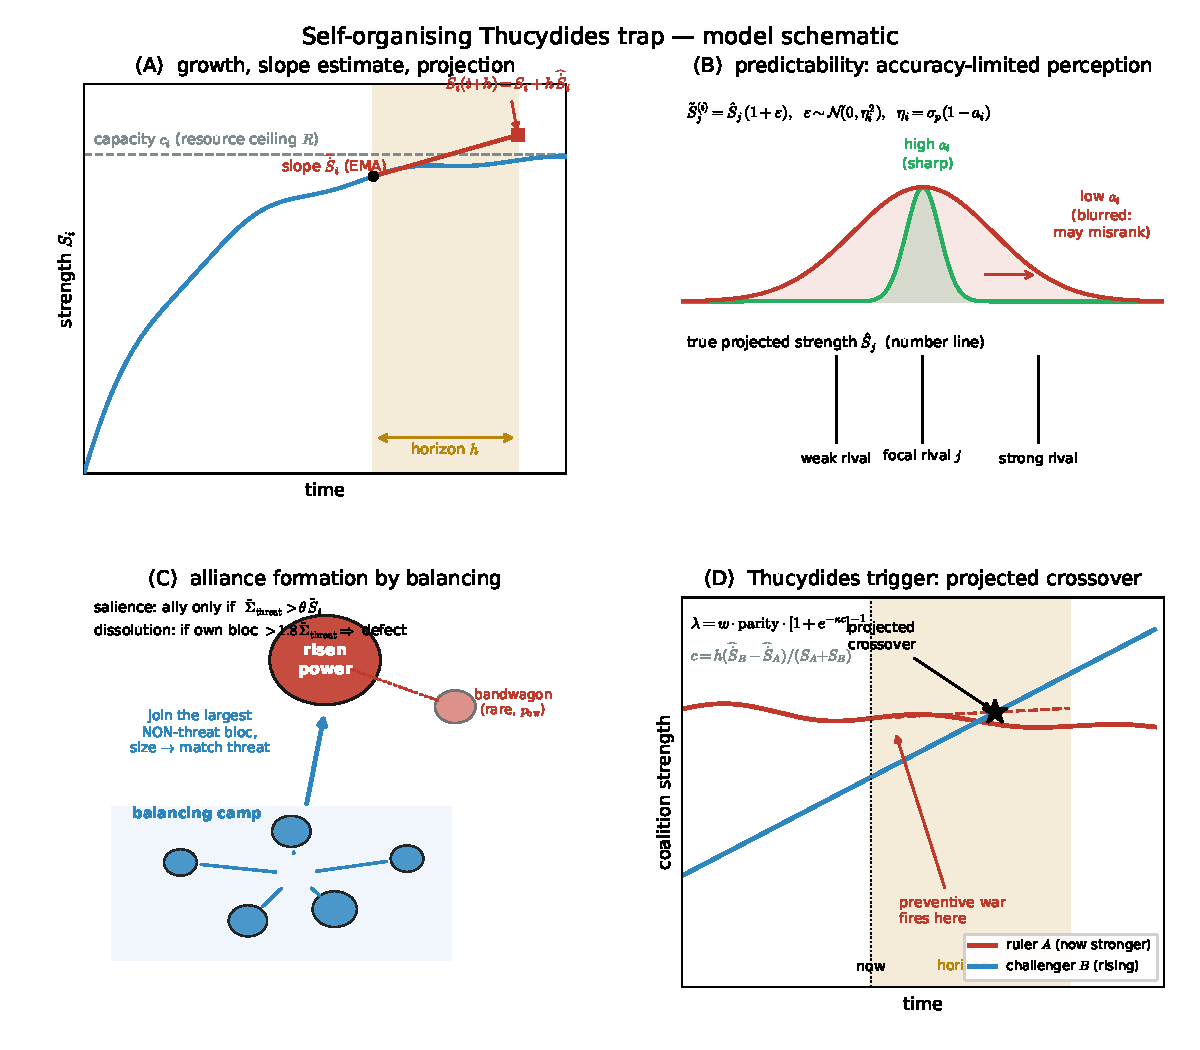
\includegraphics[width=\textwidth]{figs/selforg_schematic.pdf}
\caption{Model schematic. \textbf{(A)} Each state grows under a resource ceiling;
its trend $\widehat{\dot S}_i$ is estimated online and projected a horizon $h$
ahead to $\hat S_i(t{+}h)$. \textbf{(B)} A state perceives others' projected
strengths through accuracy-limited noise $\eta_i=\sigma_p(1-a_i)$: high $a_i$
gives a sharp estimate, low $a_i$ a blurred one that can misrank rivals.
\textbf{(C)} Balancing: a state allies only against a \emph{salient} threat,
joining the largest non-threat bloc to match it; it defects when no threat
remains; it occasionally bandwagons onto an overwhelming power. \textbf{(D)} War
ignites when a rising challenger's projected trajectory is set to cross the
ruler's within the horizon---a preventive war fired \emph{before} the crossing.}
\label{fig:schematic}
\end{figure}

\paragraph{(i) Resource-bounded stochastic growth.} It\^o, Euler--Maruyama,
\begin{equation}
dS_i=\Big[\gamma_i\,S_i\big(1-\tfrac{S_i}{c_i}\big)\,R(t)-\delta S_i\Big]dt
      +\sigma\sqrt{S_i}\,dW_i,\qquad
R(t)=\max\!\Big(0,\,1-\tfrac{\sum_j S_j}{K}\Big).
\end{equation}
Heterogeneous intrinsic rate $\gamma_i$ and per-state capacity $c_i$ (log-normal
``territory'' $\to$ a great-power/minor-power hierarchy). The global factor $R$ is
the shared-resource ceiling: no infinite growth. Demographic $\sqrt{S}$ noise
(CIR type) keeps $S\ge 0$.

\paragraph{(ii) Predictability.} ``Predictability'' has two parts: a
\emph{trend estimate} that the whole system shares, and an \emph{idiosyncratic
forecast accuracy} that differs between states and is the trait under selection.

\textbf{Trend estimate.} At the end of each round, every state's realised slope
$r_j=\big[S_j(t)-S_j(t-\Delta)\big]/\Delta$ feeds an exponential moving average
\begin{equation}
\widehat{\dot S}_j \;\leftarrow\; (1-\alpha)\,\widehat{\dot S}_j+\alpha\,r_j,
\qquad \alpha=\Delta/\tau_{\rm ema},
\end{equation}
which smooths the demographic noise to recover the underlying growth rate. The
projection a horizon $h$ ahead is the linear extrapolation
$\hat S_j=S_j+h\,\widehat{\dot S}_j$ (Fig.~\ref{fig:schematic}A). \emph{(Note the
two distinct time scales: $\Delta=n_{\rm sub}\,dt=1$ is the round length---the
clock on which the SDE is integrated and decisions are taken---whereas
$\tau_{\rm ema}=8$ is the memory of the slope filter, i.e.\ how many past rounds
are averaged; here $\alpha=\Delta/\tau_{\rm ema}=1/8$.)}

\textbf{Forecast accuracy.} Each state carries an accuracy $a_i\in(0,1]$. When $i$
needs another state's projected strength it reads it with multiplicative
Gaussian error,
\begin{equation}
\tilde S^{(i)}_j=\max\!\Big(0,\ \hat S_j\big(1+\varepsilon^{(i)}_j\big)\Big),
\qquad \varepsilon^{(i)}_j\sim\mathcal{N}\!\big(0,\eta_i^2\big),
\qquad \eta_i=\sigma_p\,(1-a_i).
\end{equation}
$a_i\!\to\!1$ is a near-perfect forecaster ($\eta\!\to\!0$); $a_i\!\to\!0$ sees
projected strengths blurred by noise of scale $\sigma_p$ and can misjudge who is
rising or who is stronger (Fig.~\ref{fig:schematic}B). \emph{Every decision below
---which threat to balance, which war to join---uses $i$'s own perceived
quantities $\tilde S^{(i)}$, never the true values.}

\textbf{Self-organisation.} $a_i$ is a heritable trait. When a state is
eliminated it respawns as the offspring of a survivor drawn with probability
$\propto S$, inheriting $a$ (and $\gamma,c$) with a small Gaussian mutation. Two
forces make $a_i$ adaptive: a good forecaster (a) joins winning coalitions and
avoids losing ones, and (b) is hard to catch unprepared---predation hazard
$\propto(1-0.85\,a_i)$ (mechanism iv). The blind are eaten, the foresighted
survive and reproduce, so $\bar a$ rises \emph{endogenously}: predictability is
selected for rather than assumed.

\paragraph{(iii) Balancing alliances.} The states are partitioned into blocs
(an alliance is a connected label set; initially all $N$ states are singletons).
Each round, every state independently reconsiders its membership with probability
$\rho$. A reconsidering state $i$ first forms the perceived strength of each bloc
$B$ from its own forecasts,
\begin{equation}
\tilde\Sigma^{(i)}_B=\sum_{j\in B}\tilde S^{(i)}_j,
\end{equation}
and identifies its \emph{top threat} as the strongest bloc it is not in,
$T=\arg\max_{B\neq b(i)}\tilde\Sigma^{(i)}_B$. It then applies four rules, in
order (Fig.~\ref{fig:schematic}C):
\begin{enumerate}
\item[\textbf{R1}] \textbf{Salience.} If the threat does not clearly outweigh
  $i$, $\tilde\Sigma^{(i)}_T<\theta\,\tilde S^{(i)}_i$, then no alliance is
  justified: if currently allied, $i$ leaves to a singleton (prob.\ $0.6$). This
  is the crux of the emergent topology---when power is diffuse \emph{no} threat
  is salient and the system stays multipolar, whereas a single risen power is a
  salient threat to \emph{many} states, who therefore converge on the \emph{same}
  balancing coalition $\Rightarrow$ bipolarity.
\item[\textbf{R2}] \textbf{Dissolution.} Else, if $i$'s own bloc already dwarfs
  the threat, $\tilde\Sigma^{(i)}_{b(i)}>1.8\,\tilde\Sigma^{(i)}_T$, the alliance
  has outlived its purpose (and dilutes the spoils): $i$ defects (prob.\ $0.6$).
  R1+R2 are what let winning coalitions \emph{fragment} after a war.
\item[\textbf{R3}] \textbf{Balancing.} Otherwise $i$ joins the bloc $B^\star$
  (excluding the threat $T$) that best matches the threat from above,
  \begin{equation}
  B^\star=\arg\max_{B\neq T}\Big[-\big|\,\Sigma^{\rm side}_B-\tilde\Sigma^{(i)}_T\,\big|
          +0.25\,\Sigma^{\rm side}_B\Big],\quad
  \Sigma^{\rm side}_B=\tilde\Sigma^{(i)}_B+\tilde S^{(i)}_i\,[\,B\neq b(i)\,],
  \end{equation}
  i.e.\ pick the camp whose strength (with $i$ added) most nearly covers the
  threat, with a mild preference for the larger camp. This is textbook
  balance-of-power: aggregate just enough weight to deter the strongest player.
\item[\textbf{R4}] \textbf{Bandwagon.} If instead the threat is overwhelming,
  $\tilde\Sigma^{(i)}_T>2.5\,\tilde S^{(i)}_i$, then with small probability
  $p_{\rm bw}$ the state \emph{joins} $T$ (a weak state buying protection from a
  hegemon rather than resisting it).
\end{enumerate}
No geography or ideology is imposed; the entire bloc structure---its size,
balance, and number---is emergent from these local rules acting on perceived
strengths.

\textbf{Alliances in war.} R1--R4 set \emph{standing} alignments; whether an ally
actually fights is a separate decision taken at war time. When lead states
$\ell_A,\ell_B$ go to war, each ally $k$ of a lead $\ell$ joins with probability
$\big[1+e^{-u_k}\big]^{-1}$, where
\begin{equation}
u_k=g\Big(P_k-\tfrac12\Big)+0.4\tanh(\tau_k-1),\quad
P_k=\frac{(\sigma^{\rm own}_k)^{q}}{(\sigma^{\rm own}_k)^{q}+(\sigma^{\rm opp}_k)^{q}},\quad
\tau_k=\frac{\sigma^{\rm opp}_k}{\tilde S^{(k)}_k},
\end{equation}
with $\sigma^{\rm own}_k=\tilde S^{(k)}_\ell+\tilde S^{(k)}_k$ and
$\sigma^{\rm opp}_k=\tilde S^{(k)}_{\ell_{\rm opp}}$: ally $k$ joins when its
\emph{own} forecast says the war is winnable ($P_k>\tfrac12$) and the opposing
side threatens it ($\tau_k>1$). A low-$a_k$ ally, mis-reading $P_k$, joins losing
wars---another channel through which predictability pays.

\paragraph{(iv) War---the Thucydides trigger.} Any sufficiently balanced pair of
blocs ($\min/\max$ strength $>0.25$) may fight, with hazard
\begin{equation}
\lambda \;=\; w\cdot
\underbrace{\tfrac{\min(S_A,S_B)}{\max(S_A,S_B)}}_{\text{parity}}
\cdot
\underbrace{\big[1+e^{-\kappa\,c}\big]^{-1}}_{\text{rising-challenger}},
\qquad c=\frac{h\,(\dot S_{\mathrm{chall}}-\dot S_{\mathrm{rul}})}{S_A+S_B},
\end{equation}
i.e.\ war fires preferentially at \textbf{parity \emph{and} when the weaker
side's projected growth is closing the gap} (preventive war against a riser;
$\widehat{\dot S}$ are the estimated slopes of the two lead states). Once
initiated between the two lead states, allies join by the war-time rule given in
(iii). Outcome is Lanchester,
$P(A)=S_A^{q}/(S_A^{q}+S_B^{q})$. The losing side pays \texttt{loss\_lose}, the
winner \texttt{loss\_win}. \textbf{Predation:} a weak \emph{unaligned} state next
to a strong bloc is conquered with hazard $\propto(1-0.85\,a_i)$---the blind get
eaten, the foresighted ally in time and survive. Eliminated states respawn weak
as singletons $\to$ continual turnover.

\paragraph{Parameters (baseline).}
Growth: $K{=}1500,\ \delta{=}0.035,\ \gamma\in[0.06,0.16],\ \sigma{=}0.16,\
c_i\sim\mathrm{LogN}(\bar c{=}12,0.6)$, round $\Delta=1$ ($n_{\rm sub}{=}5,\
dt{=}0.2$). Predictability: $\tau_{\rm ema}{=}8,\ h{=}25,\ \sigma_p{=}0.35$.
Alliances: $\rho{=}0.15,\ \theta{=}1.3,\ p_{\rm bw}{=}0.10$. War/predation:
$w{=}0.05,\ \kappa{=}12,\ q{=}1.6,\ g{=}6$, $\texttt{loss\_lose}{=}0.45,\
\texttt{loss\_win}{=}0.12$, predation rate $0.05$. Runs: $4000$ rounds.

\section{Results}

\begin{figure}[h]
\centering
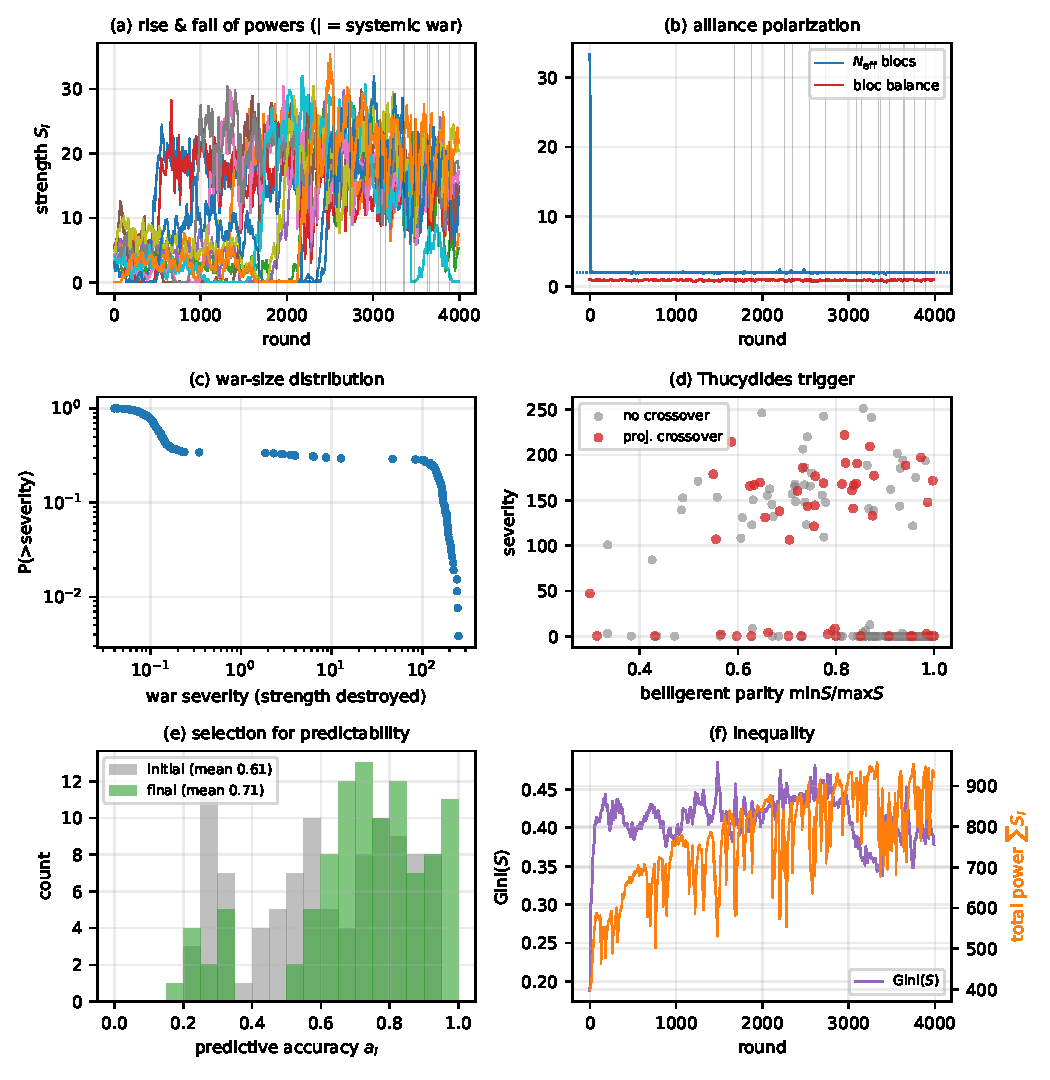
\includegraphics[width=\textwidth]{figs/selforg_overview.pdf}
\caption{(a) rise-and-fall of the strongest powers, systemic wars marked;
(b) alliance polarization $\Neff$ and bloc balance; (c) war-size CCDF;
(d) Thucydides trigger---severity vs belligerent parity, red $=$ projected
crossover; (e) selection on predictive accuracy (initial$\to$final);
(f) inequality and total power (sawtooth $=$ grow/war/regrow).}
\label{fig:overview}
\end{figure}

Aggregates over \textbf{8 seeds} (mean $\pm$ sd), with two mechanism controls:

\begin{table}[h]
\centering
\begin{tabular}{lll}
\toprule
Quantity & Baseline & Reading \\
\midrule
Effective \# blocs $\Neff$ & $\mathbf{1.99\pm0.03}$ & system self-organises to \textbf{bipolarity} \\
Bloc balance $1-\lvert f_1-f_2\rvert/(f_1+f_2)$ & $\mathbf{0.92\pm0.06}$ & the two camps are \textbf{strength-balanced} \\
Gini$(S)$ & $0.40\pm0.08$ & persistent great/minor-power hierarchy \\
Predictive accuracy $\abar$ & $\mathbf{0.58\to0.67}$ & \textbf{selected upward} (init sd only $0.03$) \\
Crossover fraction, systemic wars & $\mathbf{0.44\pm0.07}$ & systemic wars are rising-challenger wars \\
Crossover fraction, small wars & $\mathbf{0.11\pm0.03}$ & --- 4$\times$ enrichment \\
War-size distribution & heavy-tailed ($\approx$4 decades) & skirmishes $\to$ systemic wars \\
\bottomrule
\end{tabular}
\end{table}

\paragraph{Main outcomes.}
\begin{enumerate}
\item \textbf{Bipolarity is the robust attractor.} Pure self-organised balancing
  drives $\Neff\to 2$ with balanced camps, every seed. The bimodal alliance
  structure the brief hoped for \emph{is} the generic state of the system---it is
  the standing backdrop, not a rare precursor.
\item \textbf{Systemic wars are Thucydidean.} Within the bipolar structure, the
  \emph{big} wars are timed by a \textbf{projected power crossover} (rising
  challenger): $44\%$ of systemic wars carry a crossover vs $11\%$ of
  skirmishes, and systemic wars fire \emph{below} full parity ($0.75$ vs $0.90$)
  ---i.e.\ \textbf{preventively, before the challenger arrives}. Control
  $\kappa=0$ (trigger off) roughly halves the systemic-war crossover fraction
  ($0.44\to0.25$).
\item \textbf{Predictability self-organises.} Accuracy rises $0.58\to0.67$ under
  selection. Removing the explicit foresight$\to$survival coupling
  (accuracy-neutral predation) cuts the gain ($\to0.64$) but does not erase it:
  foresight also pays through better war-join decisions. Predictability is thus
  selected through \emph{several} channels, dominated by avoiding predation.
\item \textbf{Heavy-tailed war sizes $+$ rise-and-fall cycles} emerge without
  tuning (panels a, c, f): total power runs as a sawtooth---grow under the
  ceiling, systemic war resets it, regrow.
\end{enumerate}

\section{Interpretation \& novelty (literature flags)}

The pieces map onto known results---important to be honest about what is
\emph{not} new before claiming PRL novelty:
\begin{itemize}
\item \textbf{Bipolarity from balancing} is essentially Galam's spin-glass
  coalition result (Galam, \emph{Physica A} 1998/2002; Axelrod--Bennett
  ``landscape theory'' 1993, which retrodicted the WWII line-up). That balancing
  $\to$ two blocs is \emph{expected}.
\item \textbf{Power-law war sizes from a self-organising geopolitical model} is
  Cederman, \emph{APSR} 2003 (``Modeling the size of wars'', SOC)---and is
  exactly the phenomenology of the parent repo's lattice model. Not new on its
  own.
\item \textbf{Preventive war against a riser} is power-transition theory
  (Organski--Kugler 1980; Lemke), popularised as the ``Thucydides trap''
  (Allison 2017). Standard in IR, comparatively fresh as a
  \emph{dynamical-systems trigger}.
\end{itemize}

\noindent\textbf{What looks genuinely new} is the \emph{combination}: a
continuous-time \textbf{Langevin} geopolitics in which (a) \textbf{predictability
is an endogenous trait under selection}, not a fixed rationality assumption, and
(b) systemic wars are timed by a \textbf{projected-growth crossover} inside a
self-organised bipolar structure. The selection-for-foresight element---\emph{states
are pushed to become predictable because the unpredictable are eaten}---is the
part I have not seen in the physics or IR-ABM literature.

\section{Limitations of this v0}
\begin{itemize}
\item Bipolarity is \emph{too} robust ($\Neff$ pinned at 2): with no latent
  geography/ideology, balancing trivially collapses to two blocs, so the
  multipolar$\leftrightarrow$bipolar \emph{transition} (arguably the most
  interesting object) is absent. The model cannot currently show bipolarity
  \emph{emerging} before a war because it is bipolar essentially always.
\item The ``big-war'' cut ($\ge 10\%$ of world power destroyed) is a threshold,
  not an intrinsic scale; the heavy tail should be characterised as a
  distribution, not binarised.
\item Selection on $a_i$ is real but shallow ($\Delta\approx0.1$); the fitness
  gradient is parity-limited and partly hand-installed via the predation
  coupling.
\item Alliances are connected-component labels; no notion of a state in two
  alliances, of alliance \emph{reliability}, or of reputation.
\end{itemize}

\section{How to proceed (ranked)}

\paragraph{A. Make multipolar$\leftrightarrow$bipolar a real transition (highest
value).} Add a latent position $x_i$ (1-D ring or 2-D)---geography/ideology. Let
balancing prefer \emph{near} partners and threat fall off with distance. Then
regional (multipolar) blocs are the low-tension phase, and a single rising
hegemon overrides locality to force \textbf{global bipolarisation}. The order
parameter $\Neff$ then \emph{moves}, and one can ask the sharp question:
\textbf{does $\Neff\to 2$ predict the next systemic war?} This converts finding
(1) from ``always bipolar'' into a genuine precursor---the PRL hook.

\paragraph{B. Find the sharp single claim $+$ scaling law (PRL discipline).}
Two candidates:
\begin{itemize}
\item \emph{Predictability $\leftrightarrow$ stability scaling.} Sweep the
  selection strength / mean accuracy $\abar$ and measure systemic-war rate or
  mean inter-war time $\tau(\abar)$. Hypothesis: better collective foresight
  \textbf{lengthens the long peace} but \textbf{enlarges} the eventual war
  (preventive wars launched earlier, at higher stakes)---a
  predictability--severity trade-off with a clean exponent. Novel and PRL-shaped.
\item \emph{Critical line in $(w,\kappa)$} separating a ``frozen bipolar long
  peace'' from a ``churning'' phase, with diverging fluctuations / power-law
  inter-war times at the boundary (SOC vs tuned criticality---test which).
\end{itemize}

\paragraph{C. Analytics.} A 2-population mean-field (two blocs of strengths
$S_A,S_B$ under the growth SDE $+$ crossover-triggered reset) is
low-dimensional and likely tractable: a Langevin/Fokker--Planck for the gap
$g=S_A-S_B$ with an absorbing ``war'' boundary at projected crossover gives a
\textbf{first-passage} prediction for the inter-war time distribution---the
analytic backbone a PRL wants. Small-$N$ and weak-noise limits check the
simulation.

\paragraph{D. Confront data (reuse, don't rebuild).} The parent repo already
loads COW / NMC / MID. Two cheap tests: (i) does the empirical major-power system
sit near $\Neff\approx2$ before systemic wars (1914, 1939, Cold War)? (ii) is
relative-CINC \emph{slope} (rising challenger), not level, the better war
predictor---the projected-crossover claim, directly testable on NMC time series.

\paragraph{E. Cleanups.} Characterise the war-size tail (MLE power-law exponent
$+\,x_{\min}$, Clauset--Shalizi--Newman) instead of the 10\% cut; add a
reliability/defection parameter to alliances; check robustness of selection to
mutation rate.

\paragraph{Recommended first move.} \textbf{A $+$ the $\tau(\abar)$ scaling in
B}---together they turn the two lead ingredients (alliances, predictability) into
one measurable precursor and one scaling law, which is enough spine for a PRL.

\bigskip
\noindent\rule{\linewidth}{0.4pt}\\[2pt]
\noindent\textbf{Part II (the v2 model: dynamic growth, deliberation by
Monte-Carlo rollout, war-driven absorption of the loser, and the
multipolar$\leftrightarrow$bipolar transition with Options A \& B) has moved to its
own self-contained document, \texttt{NOTE\_v2.tex}.}

\end{document}
